\begin{figure}
    \centering
    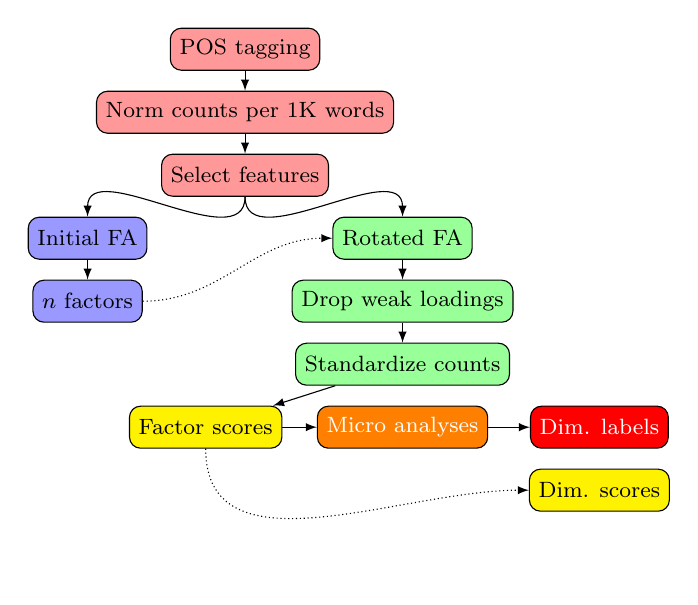
\begin{tikzpicture}
        %\tikzstyle{block} = [rectangle, rounded corners, text=black, text centered, draw=black, minimum height=.3in]
        \tikzstyle{block} = [rectangle, rounded corners, text=black, text centered, draw=black,font=\footnotesize, minimum height=.21in]
        \tikzstyle{line} = [-latex,draw=black,line width=.4]
        \node[block,fill=red!40,text=black] (tag) at (5,3) {POS tagging};
        \node[block,fill=red!40,text=black] (norm) at (5,2.2) {Norm counts per 1K words};
        \node[block,fill=red!40,text=black] (select) at (5,1.4) {Select features};
        \node[block,fill=blue!40,text=black] (fa1) at (3,.6) {Initial FA};
        \node[block,fill=blue!40,text=black] (nfactors) at (3,-.2) {$n$ factors};
        %\node[block,fill=blue!40,text=black] (comm) at (1,-.2) {Commun.};
        \node[block,fill=green!40,text=black] (fa2) at (7,.6) {Rotated FA};
        \node[block,fill=green!40,text=black] (load) at (7,-.2) {Drop weak loadings};
        \node[block,fill=green!40,text=black] (standard) at (7,-1) {Standardize counts};
        \node[block,fill=yellow,text=black] (scores) at (4.5,-1.8) {Factor scores};
        \node[block,fill=orange,text=white] (analyze) at (7,-1.8) {Micro analyses};
        \node[block,fill=red,text=white] (labels) at (9.5,-1.8) {Dim. labels};
        \node[block,fill=yellow,text=black] (dimscores) at (9.5,-2.6) {Dim. scores};
        \draw[line] (tag) to (norm);
        \draw[line] (norm) to (select);
        \draw[line] (fa1) to (nfactors);
        \draw[line] (select) to[in=90,out=270] (fa1);
        %\draw[line] (fa1) to (comm);
        \draw[line,densely dotted] (nfactors) to[in=180,out=0] (fa2);
        \draw[line] (select) to[in=90,out=270] (fa2);
        \draw[line] (fa2) to (load);
        \draw[line] (load) to (standard);
        \draw[line] (standard) to (scores);
        \draw[line] (scores) to (analyze);
        \draw[line] (analyze) to (labels);
        \draw[line, densely dotted] (scores) to[in=180,out=270] (dimscores);
        %\draw[line,densely dashed] (standard) to (labels);
        %\draw[line,loosely dashed] (standard) to (labels);
    \end{tikzpicture}
    \caption{Traditional Multi-Dimensional Analysis \citep{biberVariationSpeechWriting1988, biberDimensionsRegisterVariation1995}, \citep{berbersardinhaMultidimensionalAnalysisResearch2019, berbersardinhaMultiDimensionalAnalysis252014}}
    \label{fig:traditional_md_analysis}
\end{figure}
